\chapter{Solução Proposta e Metodologia Utilizada}

Neste capítulo será discutida a solução que foi avaliada como a mais apropriada para resolução do problema do projeto. 

O primeiro ponto a ser considerado é a metodologia de desenvolvimento da solução como um todo, vista como um problema de mineração de dados. Além disso, é feita desde uma análise detalhada dos dados utilizados e do objeto de interesse (placas de veículos), ao detalhamento do algoritmo de leitura de placas de carro que foi desenvolvido.

Também são discutidas as soluções utilizadas para adaptação do algoritmo visando a sua execução na placa Rock 3A, incluindo as tecnologias e processos necessários.

Por fim, é considerada a metodologia de teste da solução, os passos necessários para evitar viés nos resultados e garantir relevância estatística para os números obtidos.

\section{Metodologia de desenvolvimento}

A metodologia de desenvolvimento da solução como um todo segue o padrão CRISP-DM, discutido no capítulo 2, que trata o projeto como um problema de mineração de dados. Nesse padrão, o primeiro passo para o desenvolvimento do projeto é o entendimento do problema de negócio, que já foi discutido e bem definido no capítulo 3.

As etapas do projeto definidas a permitir do padrão CRISP-DM são portanto:

\begin{enumerate}
    \item \textbf{Entendimento do problema} \\
    O problema de negócio foi bem definido e explorado no capítulo 3, tendo como objetivo geral \textit{"Desenvolver um software de leitura automática de placas de veículos e validar a viabilidade funcional de uma solução de baixo custo que execute esse software em uma placa Rock 3A."}
    \item \textbf{Entendimento dos dados} \\
    Para obter um bom entendimento dos dados é necessário explorar as características tanto do \textit{dataset} utilizado quanto do objeto de interesse a ser analisado, as placas de veículos. Esse estudo será feito na próxima seção deste capítulo.
    \item \textbf{Preparação dos dados} \\
    A preparação dos dados envolve duas etapas distintas, pois esse projeto lida com dois conjuntos de dados, sendo o segundo derivado do primeiro. O primeiro conjunto são as imagens dos carros e anotações das placas, e a preparação desses dados envolve separar o \textit{dataset} em conjuntos de treino, validação e teste, além de organizá-los e transformá-los para que fiquem no padrão COCO \cite{coco}. Essa organização e transformação é necessária para que o modelo de detecção de placas seja treinado. \\ 
    A segunda etapa da preparação dos dados ocorre posteriormente e envolve a criação de um segundo conjunto de dados gerado a partir do primeiro. Esse segundo conjunto de dados deve ser um \textit{dataset} de imagens de caracteres de placas de carro, voltado para o treinamento de um modelo de classificação de caracteres. Para realização dessa tarefa, porém, é necessário que já tenha havido um avanço na modelagem, de forma que a etapa de preparação dos dados e de modelagem possuem alternância.
    \item \textbf{Modelagem} \\
    A modelagem, por sua vez, pode ser dividida em três etapas principais. A primeira é a seleção e treinamento de um modelo de detecção de objetos para a detecção das placas, etapa essa que depende da preparação do primeiro conjunto de dados, contendo as imagens dos carros e anotações das placas. \\
    A segunda etapa, que depende da primeira, é o desenvolvimento de um algoritmo para extração dos caracteres das placas identificadas pelo modelo de detecção de objetos, utilizando técnicas clássicas de visão computacional. Após essa etapa é possível (e necessária) a realização da segunda parte da preparação dos dados, que gera o \textit{dataset} de caracteres extraídos. \\
    Por fim, a última etapa de modelagem é a criação e treinamentos de modelos de redes neurais de classificação de caracteres, que devem ser capazes de identificar caracteres a partir das imagens extraídas pelo algoritmo de extração de caracteres desenvolvido.
    \item \textbf{Avaliação} \\
    A avaliação envolve realizar testes com o algoritmo completo e extrair métricas de desempenho. Esses testes devem ser realizados tanto na CPU e GPU do PC quanto na CPU e NPU da placa Rock 3A, e avaliar tanto a confiabilidade do modelo em inferir corretamente as placas dos veículos quanto a velocidade de inferência.
    \item \textbf{\textit{Deployment}} \\
    No caso deste projeto o \textit{deployment} nada mais é do que realizar um relatório final dos resultados para validar o modelo e o \textit{hardware} como viáveis ou não para o desenvolvimento de um produto de leitura automática de placas veiculares. Esse relatório estará contido no capítulo 5.
\end{enumerate}

\section{Análise dos dados}

Antes que seja possível desenvolver qualquer modelo de leitura de placas veiculares é necessário entender as características das placas a serem analisadas, além das características do \textit{dataset} específico a ser utilizado no desenvolvimento.

Nesta seção serão exploradas as diferentes variações de placas de carro existentes no Brasil que serão encontradas na nossa análise, e também os atributo dos dados a serem utilizados, como o formato das anotações e descrição da metodologia de coleta.

\subsection{Características do objeto}

O sistema de placas de carros do Brasil já passou por diversas alterações ao longo dos anos, sendo que a última mais significativa foi a adoção do "padrão Mercosul", em 2018. Desde então, dois padrões de placas veiculares seguem coexistindo, o padrão Mercosul e o padrão anterior, de 1990, que segue em circulação embora não sejam mais emitidas novas placas nesse formato.

O padrão antigo, iniciado em 1990, é um padrão alfanumérico de 7 caracteres, que seguem o formato ABC·1234. Três letras e um número de 4 dígitos, com um ponto ou hífen separando os dois blocos. 

As placas dessa modalidade costumam ser da cor cinza metálico com caracteres pretos (figura \ref{fig:placabr}), mas existem exceções importantes. Nesse padrão, algumas categorias de veículos utilizam placas de fundo colorido e caracteres brancos. A mais comum dessas categorias é a placa utilizada em veículos que realizam transporte pago, cujo fundo é vermelho (figura \ref{fig:placabrvermelha}).

\begin{figure}[H]
    \centering
    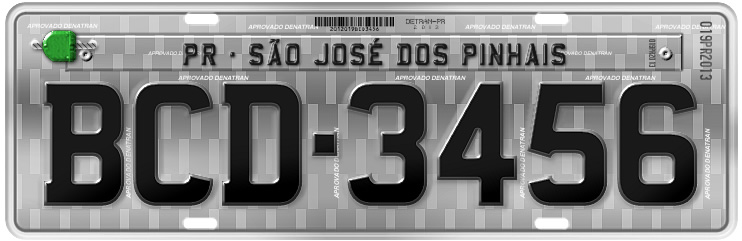
\includegraphics[width=0.8\linewidth]{images/placa-br.jpg}
    \caption{Modelo de placa veicular do Brasil de 1990}
    \label{fig:placabr}
\end{figure}

\begin{figure}[H]
    \centering
    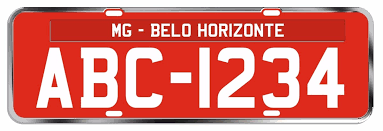
\includegraphics[width=0.8\linewidth]{images/placavermelha-br.png}
    \caption{Modelo de placa veicular do Brasil de 1990 para veículos que realizam transporte pago}
    \label{fig:placabrvermelha}
\end{figure}

As placas novas, do padrão Mercosul, utilizam uma sequência alfanumérica diferente. O formato é ABC1D23, que contém 4 letras, um número de 1 dígito e outro número de 2 dígitos, sendo que a quarta letra fica entre os dois números. Esse formato permite mais combinações diferentes que o anterior.

As placas do padrão Mercosul possuem sempre fundo branco, enquanto as letras podem variar em cor a depender da modalidade de veículo, sendo preto a mais comum (figura \ref{fig:placame}).

\begin{figure}[H]
    \centering
    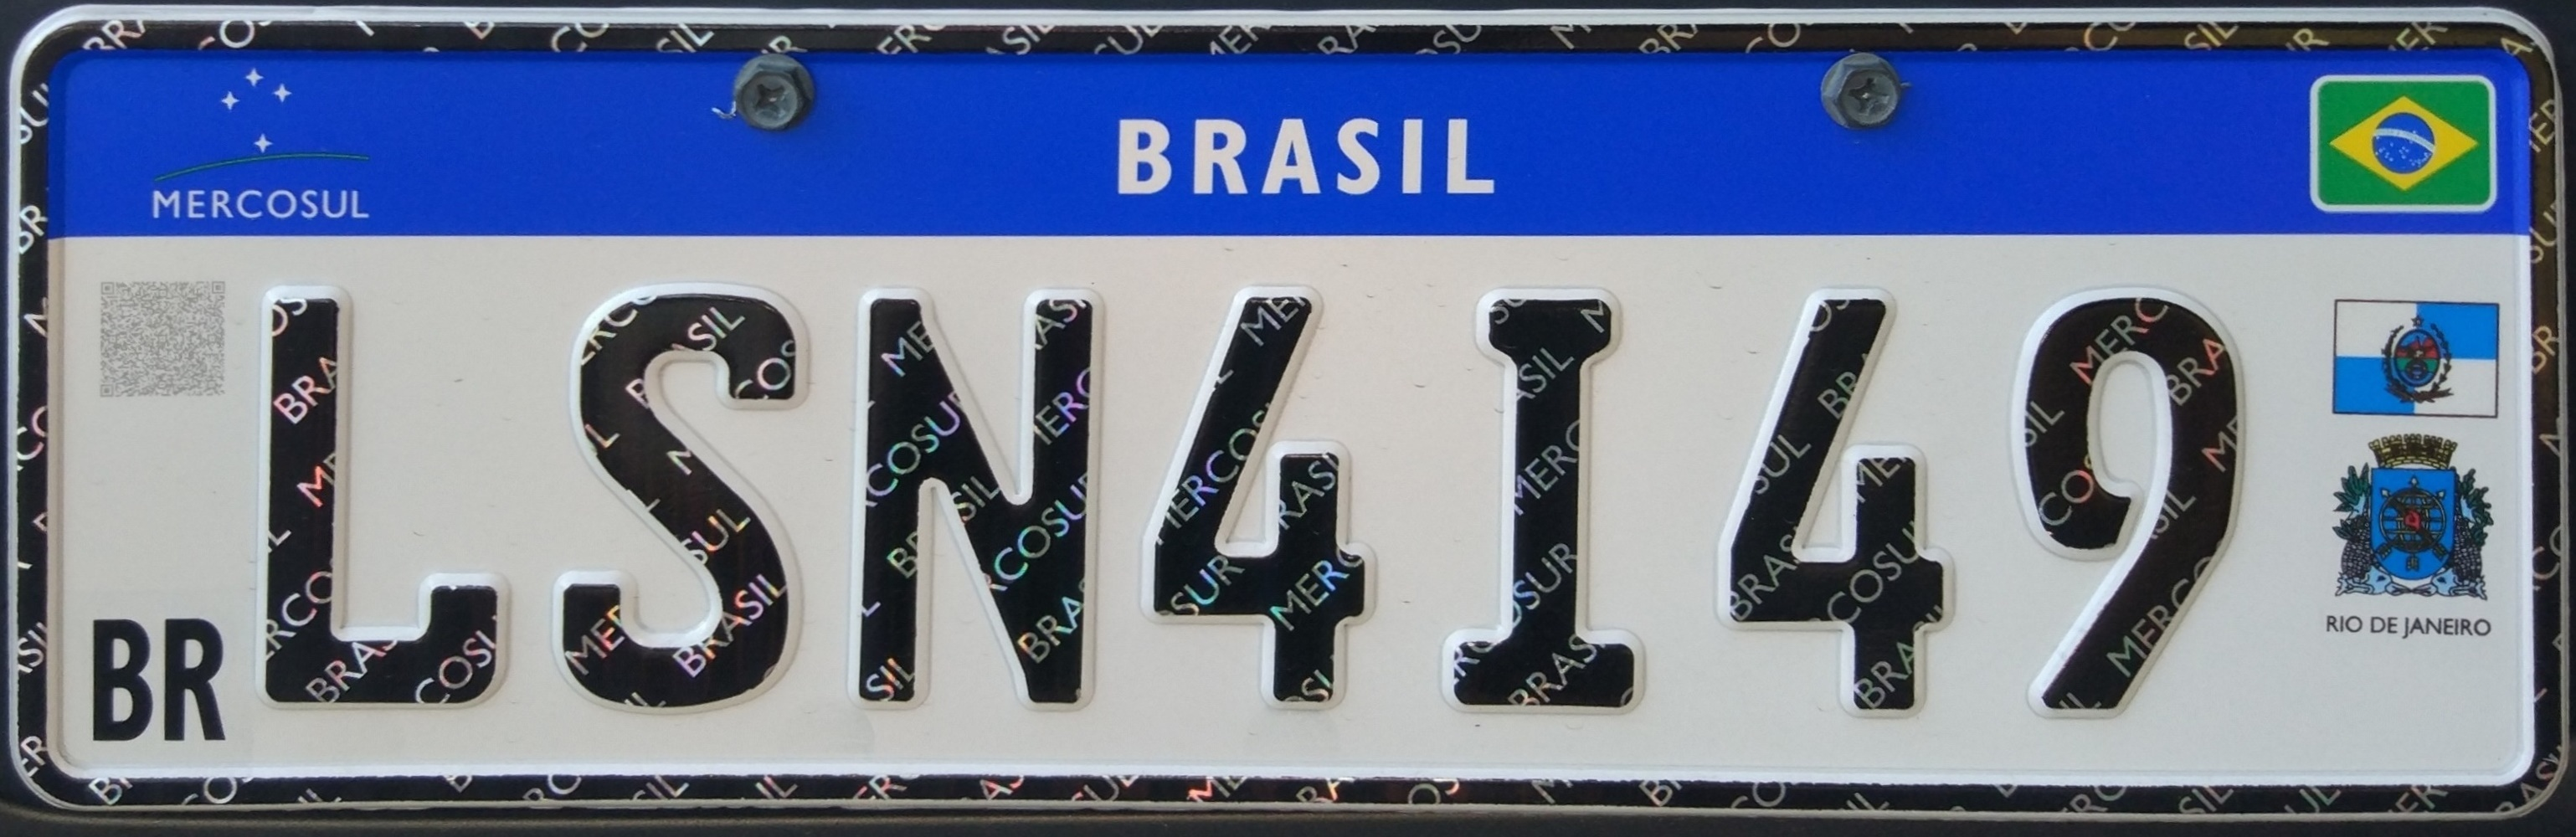
\includegraphics[width=0.8\linewidth]{images/placa-me.jpg}
    \caption{Modelo de placa veicular do padrão Mercosul}
    \label{fig:placame}
\end{figure}

Ambos modelos de placas possuem informações adicionais na parte de cima, notadamente o padrão de 1990 inclui a cidade e UF do veículo e o padrão Mercosul inclui o país. Além disso, as placas do padrão Mercosul incluem símbolos e selos adicionais que ajudam na verificação de autenticidade. Os dois modelos possuem margens ao redor do texto principal.

\subsection{Características do \textit{dataset} utilizado}

O conjunto de dados utilizado foi RodoSol-ALPR, criado no trabalho \cite{dataset}. Esse \textit{dataset} é composto por 10.000 imagens de carros e 10.000 imagens de motocicletas com dimensão de 1.280 x 720 px. As imagens, além de serem classificadas como "carro" ou "moto", também são classificadas entre veículos com placa no padrão antigo (BR) e com placa no padrão Mercosul (ME), sendo que metade das imagens tanto de carros quanto de motos pertencem a cada padrão de placa.

As imagens desse \textit{dataset} foram capturadas por câmeras estáticas em um pedágio na Rodovia do Sol, no Espírito Santo. Inclui imagens com iluminação boa e ruim, com chuva e sem, além de carros em diferentes distancias da câmera.

As anotações das imagens são no seguinte formato:

\begin{verbatim}
type: car
plate: ODE2510
layout: Brazilian
corners: 558,438 687,439 687,482 558,481
\end{verbatim}

A primeira linha especifica o tipo de veículo (\textit{car/motorcycle}), a segunda, os caracteres da placa, a terceira o layout da placa (\textit{Brazilian/Mercosur}) e a quarta as coordenadas dos 4 cantos da placa em pixels.

A figura \ref{fig:inputexemplo} é um exemplo de imagem do \textit{dataset} com as marcações dos 4 cantos da placa obtidas do arquivo de anotação.

\begin{figure}[H]
    \centering
    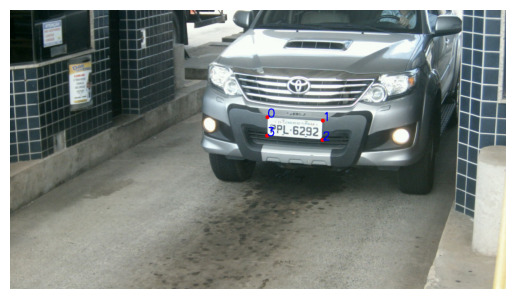
\includegraphics[width=0.8\linewidth]{images/exemplo-input.png}
    \caption{Exemplo de imagem do \textit{dataset} com as marcações dos 4 cantos da placa}
    \label{fig:inputexemplo}
\end{figure}

\section{\textit{Pipeline} de leitura de placas}



\section{Modelo de detecção de objetos}

\section{Algoritmo de extração de caracteres}

\section{Modelos de classificação de caracteres}

\section{Conversão para execução na placa Rock 3A}

\section{Metodologia de teste}